
%% bare_conf.tex
%% V1.4b
%% 2015/08/26
%% by Michael Shell
%% See:
%% http://www.michaelshell.org/
%% for current contact information.
%%
%% This is a skeleton file demonstrating the use of IEEEtran.cls
%% (requires IEEEtran.cls version 1.8b or later) with an IEEE
%% conference paper.
%%
%% Support sites:
%% http://www.michaelshell.org/tex/ieeetran/
%% http://www.ctan.org/pkg/ieeetran
%% and
%% http://www.ieee.org/

%%*************************************************************************
%% Legal Notice:
%% This code is offered as-is without any warranty either expressed or
%% implied; without even the implied warranty of MERCHANTABILITY or
%% FITNESS FOR A PARTICULAR PURPOSE! 
%% User assumes all risk.
%% In no event shall the IEEE or any contributor to this code be liable for
%% any damages or losses, including, but not limited to, incidental,
%% consequential, or any other damages, resulting from the use or misuse
%% of any information contained here.
%%
%% All comments are the opinions of their respective authors and are not
%% necessarily endorsed by the IEEE.
%%
%% This work is distributed under the LaTeX Project Public License (LPPL)
%% ( http://www.latex-project.org/ ) version 1.3, and may be freely used,
%% distributed and modified. A copy of the LPPL, version 1.3, is included
%% in the base LaTeX documentation of all distributions of LaTeX released
%% 2003/12/01 or later.
%% Retain all contribution notices and credits.
%% ** Modified files should be clearly indicated as such, including  **
%% ** renaming them and changing author support contact information. **
%%*************************************************************************


% *** Authors should verify (and, if needed, correct) their LaTeX system  ***
% *** with the testflow diagnostic prior to trusting their LaTeX platform ***
% *** with production work. The IEEE's font choices and paper sizes can   ***
% *** trigger bugs that do not appear when using other class files.       ***                          ***
% The testflow support page is at:
% http://www.michaelshell.org/tex/testflow/



\documentclass[conference]{IEEEtran}
% Some Computer Society conferences also require the compsoc mode option,
% but others use the standard conference format.
%
% If IEEEtran.cls has not been installed into the LaTeX system files,
% manually specify the path to it like:
% \documentclass[conference]{../sty/IEEEtran}





% Some very useful LaTeX packages include:
% (uncomment the ones you want to load)


% *** MISC UTILITY PACKAGES ***
%
%\usepackage{ifpdf}
% Heiko Oberdiek's ifpdf.sty is very useful if you need conditional
% compilation based on whether the output is pdf or dvi.
% usage:
% \ifpdf
%   % pdf code
% \else
%   % dvi code
% \fi
% The latest version of ifpdf.sty can be obtained from:
% http://www.ctan.org/pkg/ifpdf
% Also, note that IEEEtran.cls V1.7 and later provides a builtin
% \ifCLASSINFOpdf conditional that works the same way.
% When switching from latex to pdflatex and vice-versa, the compiler may
% have to be run twice to clear warning/error messages.


\usepackage{subcaption}



% *** CITATION PACKAGES ***
%
\usepackage{cite}
% cite.sty was written by Donald Arseneau
% V1.6 and later of IEEEtran pre-defines the format of the cite.sty package
% \cite{} output to follow that of the IEEE. Loading the cite package will
% result in citation numbers being automatically sorted and properly
% "compressed/ranged". e.g., [1], [9], [2], [7], [5], [6] without using
% cite.sty will become [1], [2], [5]--[7], [9] using cite.sty. cite.sty's
% \cite will automatically add leading space, if needed. Use cite.sty's
% noadjust option (cite.sty V3.8 and later) if you want to turn this off
% such as if a citation ever needs to be enclosed in parenthesis.
% cite.sty is already installed on most LaTeX systems. Be sure and use
% version 5.0 (2009-03-20) and later if using hyperref.sty.
% The latest version can be obtained at:
% http://www.ctan.org/pkg/cite
% The documentation is contained in the cite.sty file itself.






% *** GRAPHICS RELATED PACKAGES ***
%
\ifCLASSINFOpdf
  \usepackage[pdftex]{graphicx}
  % declare the path(s) where your graphic files are
  % \graphicspath{{../pdf/}{../jpeg/}}
  % and their extensions so you won't have to specify these with
  % every instance of \includegraphics
  % \DeclareGraphicsExtensions{.pdf,.jpeg,.png}
\else
  % or other class option (dvipsone, dvipdf, if not using dvips). graphicx
  % will default to the driver specified in the system graphics.cfg if no
  % driver is specified.
  % \usepackage[dvips]{graphicx}
  % declare the path(s) where your graphic files are
  % \graphicspath{{../eps/}}
  % and their extensions so you won't have to specify these with
  % every instance of \includegraphics
  % \DeclareGraphicsExtensions{.eps}
\fi
% graphicx was written by David Carlisle and Sebastian Rahtz. It is
% required if you want graphics, photos, etc. graphicx.sty is already
% installed on most LaTeX systems. The latest version and documentation
% can be obtained at: 
% http://www.ctan.org/pkg/graphicx
% Another good source of documentation is "Using Imported Graphics in
% LaTeX2e" by Keith Reckdahl which can be found at:
% http://www.ctan.org/pkg/epslatex
%
% latex, and pdflatex in dvi mode, support graphics in encapsulated
% postscript (.eps) format. pdflatex in pdf mode supports graphics
% in .pdf, .jpeg, .png and .mps (metapost) formats. Users should ensure
% that all non-photo figures use a vector format (.eps, .pdf, .mps) and
% not a bitmapped formats (.jpeg, .png). The IEEE frowns on bitmapped formats
% which can result in "jaggedy"/blurry rendering of lines and letters as
% well as large increases in file sizes.
%
% You can find documentation about the pdfTeX application at:
% http://www.tug.org/applications/pdftex





% *** MATH PACKAGES ***
%
\usepackage{amsmath}
\usepackage{mathabx}
% A popular package from the American Mathematical Society that provides
% many useful and powerful commands for dealing with mathematics.
%
% Note that the amsmath package sets \interdisplaylinepenalty to 10000
% thus preventing page breaks from occurring within multiline equations. Use:
%\interdisplaylinepenalty=2500
% after loading amsmath to restore such page breaks as IEEEtran.cls normally
% does. amsmath.sty is already installed on most LaTeX systems. The latest
% version and documentation can be obtained at:
% http://www.ctan.org/pkg/amsmath





% *** SPECIALIZED LIST PACKAGES ***
%
%\usepackage{algorithmic}
% algorithmic.sty was written by Peter Williams and Rogerio Brito.
% This package provides an algorithmic environment fo describing algorithms.
% You can use the algorithmic environment in-text or within a figure
% environment to provide for a floating algorithm. Do NOT use the algorithm
% floating environment provided by algorithm.sty (by the same authors) or
% algorithm2e.sty (by Christophe Fiorio) as the IEEE does not use dedicated
% algorithm float types and packages that provide these will not provide
% correct IEEE style captions. The latest version and documentation of
% algorithmic.sty can be obtained at:
% http://www.ctan.org/pkg/algorithms
% Also of interest may be the (relatively newer and more customizable)
% algorithmicx.sty package by Szasz Janos:
% http://www.ctan.org/pkg/algorithmicx




% *** ALIGNMENT PACKAGES ***
%
%\usepackage{array}
% Frank Mittelbach's and David Carlisle's array.sty patches and improves
% the standard LaTeX2e array and tabular environments to provide better
% appearance and additional user controls. As the default LaTeX2e table
% generation code is lacking to the point of almost being broken with
% respect to the quality of the end results, all users are strongly
% advised to use an enhanced (at the very least that provided by array.sty)
% set of table tools. array.sty is already installed on most systems. The
% latest version and documentation can be obtained at:
% http://www.ctan.org/pkg/array


% IEEEtran contains the IEEEeqnarray family of commands that can be used to
% generate multiline equations as well as matrices, tables, etc., of high
% quality.




% *** SUBFIGURE PACKAGES ***
%\ifCLASSOPTIONcompsoc
%  \usepackage[caption=false,font=normalsize,labelfont=sf,textfont=sf]{subfig}
%\else
%  \usepackage[caption=false,font=footnotesize]{subfig}
%\fi
% subfig.sty, written by Steven Douglas Cochran, is the modern replacement
% for subfigure.sty, the latter of which is no longer maintained and is
% incompatible with some LaTeX packages including fixltx2e. However,
% subfig.sty requires and automatically loads Axel Sommerfeldt's caption.sty
% which will override IEEEtran.cls' handling of captions and this will result
% in non-IEEE style figure/table captions. To prevent this problem, be sure
% and invoke subfig.sty's "caption=false" package option (available since
% subfig.sty version 1.3, 2005/06/28) as this is will preserve IEEEtran.cls
% handling of captions.
% Note that the Computer Society format requires a larger sans serif font
% than the serif footnote size font used in traditional IEEE formatting
% and thus the need to invoke different subfig.sty package options depending
% on whether compsoc mode has been enabled.
%
% The latest version and documentation of subfig.sty can be obtained at:
% http://www.ctan.org/pkg/subfig




% *** FLOAT PACKAGES ***
%
%\usepackage{fixltx2e}
% fixltx2e, the successor to the earlier fix2col.sty, was written by
% Frank Mittelbach and David Carlisle. This package corrects a few problems
% in the LaTeX2e kernel, the most notable of which is that in current
% LaTeX2e releases, the ordering of single and double column floats is not
% guaranteed to be preserved. Thus, an unpatched LaTeX2e can allow a
% single column figure to be placed prior to an earlier double column
% figure.
% Be aware that LaTeX2e kernels dated 2015 and later have fixltx2e.sty's
% corrections already built into the system in which case a warning will
% be issued if an attempt is made to load fixltx2e.sty as it is no longer
% needed.
% The latest version and documentation can be found at:
% http://www.ctan.org/pkg/fixltx2e


%\usepackage{stfloats}
% stfloats.sty was written by Sigitas Tolusis. This package gives LaTeX2e
% the ability to do double column floats at the bottom of the page as well
% as the top. (e.g., "\begin{figure*}[!b]" is not normally possible in
% LaTeX2e). It also provides a command:
%\fnbelowfloat
% to enable the placement of footnotes below bottom floats (the standard
% LaTeX2e kernel puts them above bottom floats). This is an invasive package
% which rewrites many portions of the LaTeX2e float routines. It may not work
% with other packages that modify the LaTeX2e float routines. The latest
% version and documentation can be obtained at:
% http://www.ctan.org/pkg/stfloats
% Do not use the stfloats baselinefloat ability as the IEEE does not allow
% \baselineskip to stretch. Authors submitting work to the IEEE should note
% that the IEEE rarely uses double column equations and that authors should try
% to avoid such use. Do not be tempted to use the cuted.sty or midfloat.sty
% packages (also by Sigitas Tolusis) as the IEEE does not format its papers in
% such ways.
% Do not attempt to use stfloats with fixltx2e as they are incompatible.
% Instead, use Morten Hogholm'a dblfloatfix which combines the features
% of both fixltx2e and stfloats:
%
% \usepackage{dblfloatfix}
% The latest version can be found at:
% http://www.ctan.org/pkg/dblfloatfix




% *** PDF, URL AND HYPERLINK PACKAGES ***
%
\usepackage{url}
% url.sty was written by Donald Arseneau. It provides better support for
% handling and breaking URLs. url.sty is already installed on most LaTeX
% systems. The latest version and documentation can be obtained at:
% http://www.ctan.org/pkg/url
% Basically, \url{my_url_here}.


%\usepackage{asmfonts}

% *** Do not adjust lengths that control margins, column widths, etc. ***
% *** Do not use packages that alter fonts (such as pslatex).         ***
% There should be no need to do such things with IEEEtran.cls V1.6 and later.
% (Unless specifically asked to do so by the journal or conference you plan
% to submit to, of course. )


% correct bad hyphenation here
\hyphenation{op-tical net-works semi-conduc-tor}


\begin{document}
%
% paper title
% Titles are generally capitalized except for words such as a, an, and, as,
% at, but, by, for, in, nor, of, on, or, the, to and up, which are usually
% not capitalized unless they are the first or last word of the title.
% Linebreaks \\ can be used within to get better formatting as desired.
% Do not put math or special symbols in the title.
\title{Semantic Holographic Memories}


% author names and affiliations
% use a multiple column layout for up to three different
% affiliations
\author{\IEEEauthorblockN{Igor Peric, Stefan Ulbrich, Alexandru Lesi, R{\"u}diger Dillman, Marius Z{\"o}llner}
\IEEEauthorblockA{FZI Forschungszentrum Informatik\\
Karlsruhe, Germany\\
Email: $\{$peric, ulbrich, dillmann, zoellner$\}$@fzi.de}
}

% conference papers do not typically use \thanks and this command
% is locked out in conference mode. If really needed, such as for
% the acknowledgment of grants, issue a \IEEEoverridecommandlockouts
% after \documentclass

% for over three affiliations, or if they all won't fit within the width
% of the page, use this alternative format:
% 
%\author{\IEEEauthorblockN{Michael Shell\IEEEauthorrefmark{1},
%Homer Simpson\IEEEauthorrefmark{2},
%James Kirk\IEEEauthorrefmark{3}, 
%Montgomery Scott\IEEEauthorrefmark{3} and
%Eldon Tyrell\IEEEauthorrefmark{4}}
%\IEEEauthorblockA{\IEEEauthorrefmark{1}School of Electrical and Computer Engineering\\
%Georgia Institute of Technology,
%Atlanta, Georgia 30332--0250\\ Email: see http://www.michaelshell.org/contact.html}
%\IEEEauthorblockA{\IEEEauthorrefmark{2}Twentieth Century Fox, Springfield, USA\\
%Email: homer@thesimpsons.com}
%\IEEEauthorblockA{\IEEEauthorrefmark{3}Starfleet Academy, San Francisco, California 96678-2391\\
%Telephone: (800) 555--1212, Fax: (888) 555--1212}
%\IEEEauthorblockA{\IEEEauthorrefmark{4}Tyrell Inc., 123 Replicant Street, Los Angeles, California 90210--4321}}


% use for special paper notices
%\IEEEspecialpapernotice{(Invited Paper)}


% make the title area
\maketitle

% As a general rule, do not put math, special symbols or citations
% in the abstract
\begin{abstract}
Vector Symbolic Architectures (VSA) define a set of operations for storage (compression), manipulation and retrieval of symbolic concepts, represented as fixed-length vectors. A specific instance of VSA, Holographic Reduced Representations (HRR), has proven to exhibit properties similar to human short-term memory and is, as such, interesting for computational modeling.

In this paper we extend HRR approach by introducing topology-preserving, invertible encoding/decoding procedure for all major data types used in robotics and engineering. These encoding schemes play the role of otherwise used clean-up modules after memory retrieval (e.g. self-organizing maps), thus eliminating necessity for them.

We test our memories in three different robotic tasks: mapping and recall, visual object classification and state machine scripting (holographic controllers).
\end{abstract}

% no keywords




% For peer review papers, you can put extra information on the cover
% page as needed:
% \ifCLASSOPTIONpeerreview
% \begin{center} \bfseries EDICS Category: 3-BBND \end{center}
% \fi
%
% For peerreview papers, this IEEEtran command inserts a page break and
% creates the second title. It will be ignored for other modes.
\IEEEpeerreviewmaketitle



\section{Introduction}

Vector Symbolic Architectures (VSA) define a set of operations for storage (compression) and retrieval of symbolic concepts in fixed size vectors. In its basic form every VSA has to implement three basic operations:
\begin{enumerate}
\item association (binding) $\mapsto \otimes$
\item superposition (appending) $\mapsto +$
\item probing (unbinding) $\mapsto \oslash$
\end{enumerate}

In addition, every VSA can be considered as a compression technique, since binary operations on N-element vectors return N-element vectors as well.

\textbf{Association} (also called "binding") is operation of linking two operands together, resulting in a vector of same size which is dissimilar (orthogonal) to both original vectors, but contains scrambled information from both of the operands. For instance, linking property "red" to object "triangle" can be done using binding operation:

\begin{equation}
memory_1 = red \otimes triangle
\end{equation}

\textbf{Superposition} is operation of extending a set of already memorized items with another item (or binding of two or more of them). As an example, a memory of "red triangle and blue circle" can be formed in following way:
\begin{equation}
memory_2 = memory_1 + blue \otimes circle
\end{equation}

\textbf{Probing} is operation of extracting a noisy version of associated item from a joint set memory. I.e. a question "What is the color of triangle?" could be asked like this:

\begin{equation}
red \approx memory_2 \oslash triangle
\end{equation}

Probing operation assumes existence of inverse element to association, so previous equation can be interpreted and explained in following way:
\begin{multline}
memory_2 \otimes triangle'=\\
(red \otimes triangle + blue \otimes circle) \otimes triangle'=\\
red \otimes triangle  \otimes triangle' + blue \otimes circle \otimes triangle' =\\
red + blue \otimes circle \otimes triangle'  = red + noise
\approx red
\end{multline}

where $triangle'$ represents inverse of $triangle$. Resulting vector will be composition of something that is very similar to $red$ and something that doesn't resemble anything meaningful from symbol table, so it can be treated as neglectable noise.

\begin{figure}
\center
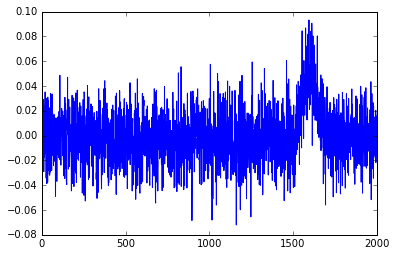
\includegraphics[width=0.9\columnwidth]{img/scalar-probe.png}
\caption{Result of $(80 \otimes A) \oslash A$ for HRR from}
\end{figure}

Process of converting noisy result of probing into the closest know symbol is called \textbf{clean-up procedure}. Straightforward way of implementing clean-up memory is using lookup table, while other researchers show that any type of attractor network can be used (e.g. self-organizing maps).

\section{Holographic reduced representations}


Holographic Reduced Representations are VSAs which implement operation of binding as circular convolution:

\begin{equation}
z_i=\sum_{k=0}^{N}{x_iy_{i-k}} //TODO
\end{equation}

where $z$ is the result of convolution, $x$ and $y$ are operands of size $N$. Superposition is implemented as simple element-wise addition. Probing is implemented using inverse of circular convolution - circular correlation:

\begin{equation}
y_i=\sum_{k=0}^{m}{x_iy_{i-k}} //TODO
\end{equation} 

- Implementation and building up of HRRs (similarity measures and cosine, lookup table...)


\section{Topology-preserving encoding}

- necessity (benefit of having it, querying smth that was not there)
- implementation

In order to use various types of inputs with HRRs it is necessary to encode them in vectors of fixed size. The basic approach is to generate these vectors randomly for each distinct input and store these pairs in a map. This will consequently take its toll on the space complexity and may become infeasible, depending on the type of input used. The following section presents ways to encode values in a deterministic manner, removing the need to store these, as long as decoding is robust against noise. 

\subsection{Scalars}

Encoding scalars is a good example for the necessity of preserving topology. Depending on what dataset is in use it may be required to store mappings for any number of values. Furthermore, using random encoding, there would be no similarity in neighbouring values. As such the following probe will yield no result:

\begin{equation}
(10000 \otimes A) \oslash 10001
\end{equation}

To facilitate these two qualities scalar encoding can be achieved with the help of Gaussian distributions. The encoded vector will simply represent a Gaussian bell sampled over a fixed input range. Figure \ref{no-perm-a} shows how such an encoded vector looks like, and what the result of binding it to a generic random vector is. With this result it becomes obvious that lots of information is lost. If this result is probed with the same random vector used in binding something similar to the initial Gaussian bell is expected. And yet figure \ref{no-perm-b} presents no such outcome. While there is a peak at the initial value lots of other peaks also arise, making it impossible to detect which one is correct. 

\begin{figure}
\begin{subfigure}{1\columnwidth}
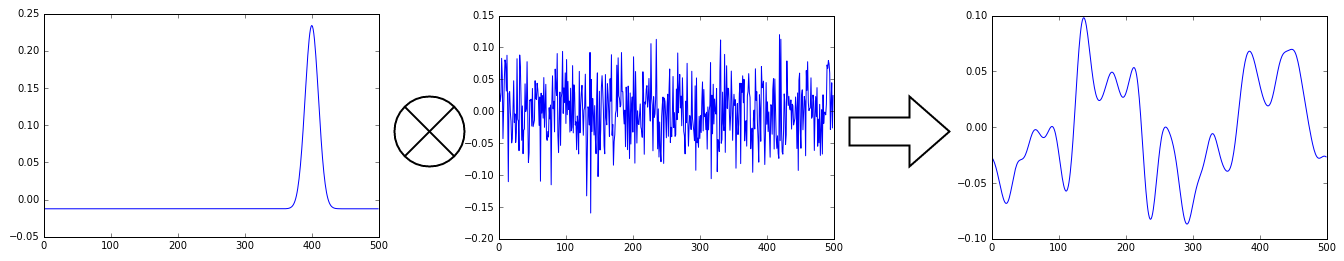
\includegraphics[width=\columnwidth]{img/scalar-pre-perm.png}
\caption{Binging}
\label{no-perm-a}
\end{subfigure}
\begin{subfigure}{1\columnwidth}
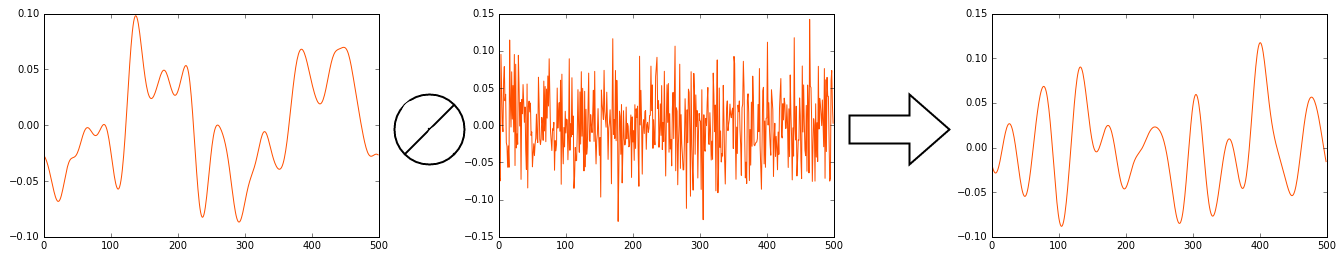
\includegraphics[width=\columnwidth]{img/scalar-pre-perm-probe.png}
\caption{Probing}
\label{no-perm-b}
\end{subfigure}
\caption{Plot of vector values. Figure \ref{no-perm-a} shows the binding of the value 8 on a scale to 10 with the symbolic representation of "ball", which is random. In figure \ref{no-perm-b} "ball" is being probed, and the expected result is a Gaussian bell for 8, mixed with some noise.}
\label{no-perm}
\end{figure}

This effect is due to the fact that circular convolution is based on Fourier transformations and the lack of frequencies present in encoded vectors becomes apparent in Fourier space as well. Figure \ref{fft} highlights this. All the information of a Gaussian bell is crammed into the lowest and highest values of the Fourier transformation. In these circumstances, when probing for a scalar, the vector received is in turn recreated of too few frequencies and does not come close to resembling the original Gaussian. 

\begin{figure}
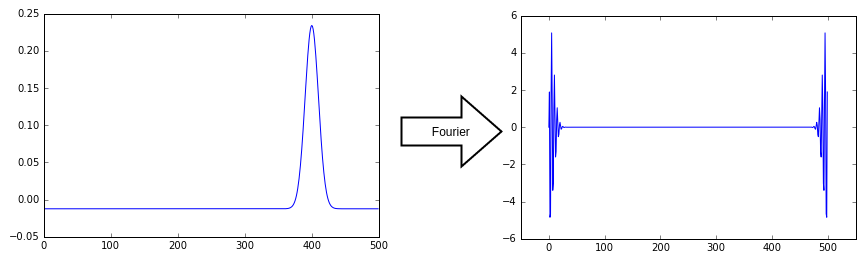
\includegraphics[width=\columnwidth]{img/scalar-pre-perm-fft.png}
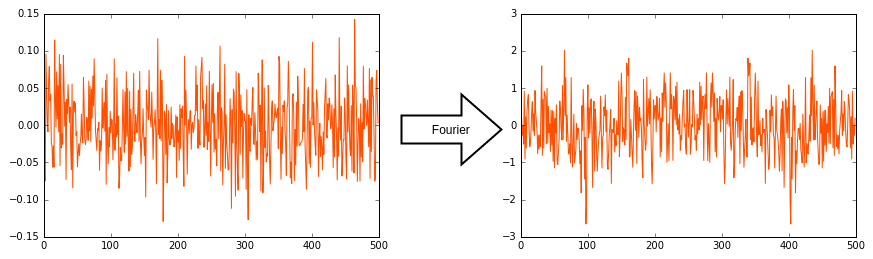
\includegraphics[width=\columnwidth]{img/scalar-random-fft.png}
\caption{Fourier space conversions of a Gaussian bell and a random vector.}
\label{fft}
\end{figure}

This inconvenience is removed with the help of permutations. Depending on the size of the memory vectors used a fixed permutation is generated. Whenever a scalar is encoded the Gaussian bell is first sampled over the range, after which the sampled values swap places accordingly. As such the resulting vector will present lots of jumps in value, which have a significant impact on the Fourier space, as can be seen in figure \ref{perm-fft}.

\begin{figure}
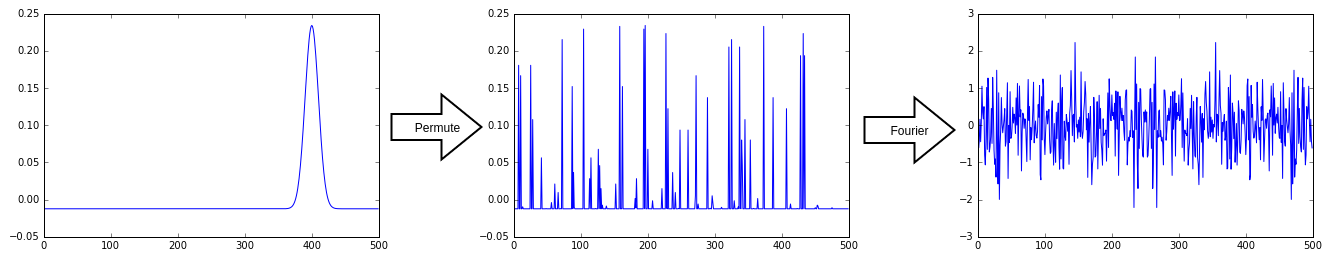
\includegraphics[width=\columnwidth]{img/scalar-perm-step-fft.png}
\caption{Plots on the effect of permuting a Gaussian bell, and the impact on Fourier space.}
\label{perm-fft}
\end{figure}

Working with such a vector makes it possible to successfully probe for scalars and receive a Gaussian bell overlapped with some noise. All of this can be seen in figure \ref{perm}, which depicts the exact same operations as figure \ref{no-perm}, but using a permuted version of a Gaussian bell. The result in figure \ref{perm-b} clearly shows an according spike. This vector can be smoothed out, after which the peak can easily be identified and the initial scalar can be recovered.

\begin{figure}
\begin{subfigure}{1\columnwidth}
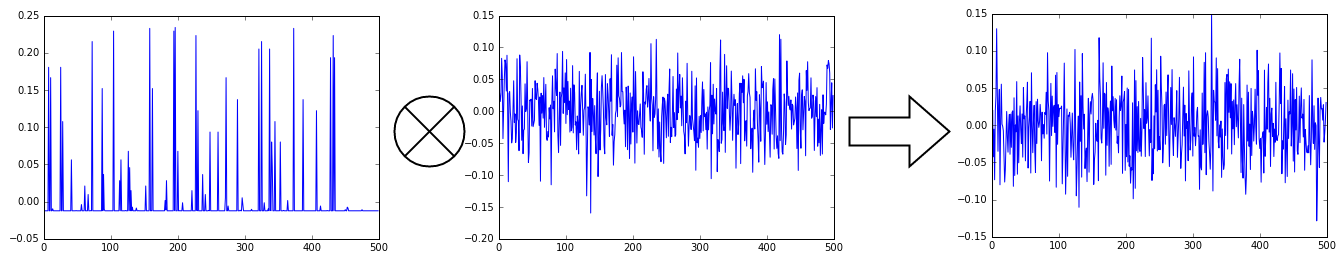
\includegraphics[width=\columnwidth]{img/scalar-post-perm.png}
\caption{Binging}
\label{perm-a}
\end{subfigure}
\begin{subfigure}{1\columnwidth}
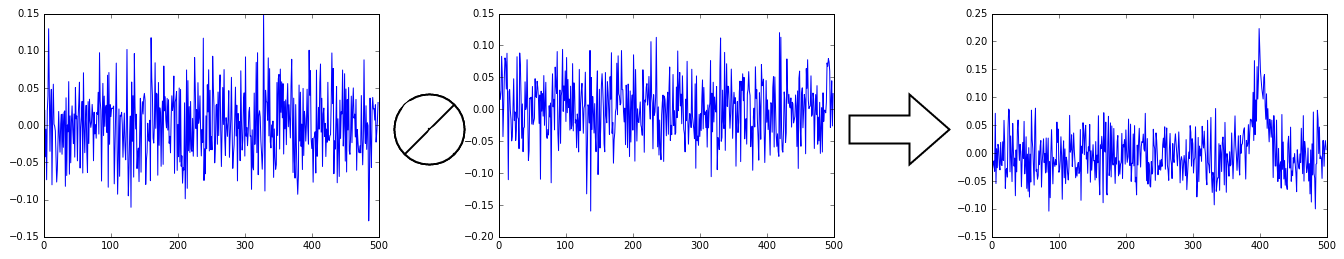
\includegraphics[width=\columnwidth]{img/scalar-post-perm-probe.png}
\caption{Probing}
\label{perm-b}
\end{subfigure}
\caption{Figure \ref{perm-a} shows the binding of the permuted Gaussian for value 8 on a scale to 10 with the symbolic representation of "ball", which is random. In figure \ref{perm-b} "ball" is being probed, and the expected result is a Gaussian bell for 8, mixed with some noise.}
\label{perm}
\end{figure}

On a technical note it became apparent that simply sampling Gaussian bells in a vector with all the values greater zero brought up a small issue. Adding multiple such bindings on top of each other would constantly increase the values in the resulting vector. Due to this, when probing, we would receive vectors which had the correct distance between their values, i.e. the correct "shape", but would be shifted on the Y-axis. This can be solved by editing the permuted Gaussian bell to have \(\sum_{i=0}^n x_i = 0\), and is achieved with this simple operation:

\[ \forall x_i \in x: x_i = x_i - \frac{\sum_{i=0}^n ||x_i||}{|x|} \]

\subsection{Coordinate encoder}

\subsection{String encoder}

\section{Properties of SHM}

- you can't extract the items memorized, number of them, you can just query
- they are probabilistic
- you can modify them online (no separate learning/probing phases)
\subsection{Capacity}
\subsubsection{SHM size vs. number of items}
\subsubsection{Model of human forgetting}
\subsubsection{Model of intentional forgetting}

\subsection{Fan-out effect - multiple probing outputs}

\subsection{Limitations}

- introducing problem of lookup (symbol grounding)
- solution using implicit encoding and decoding

\section{Experiments}

\subsection{Visual object classification}
- SIFT + label
\subsection{Localization and mapping}
- SIFT + location
\subsection{Holographic state machines (holographic controllers)}
- sensory\_data + current\_state + next state
\subsection{Reinforcement learning}
- sensory\_data + action + reward
\subsection{Language understanding}
- TensorFlow (role) + word = question answering
\subsection{Implicit inductive reasoning}

\section{Conclusions}


% use section* for acknowledgment
\section*{Acknowledgment}

% leaving this as is.
The authors would like to thank... Manchester developers. :slowclap:


\bibliographystyle{IEEEtran}
 
\bibliography{IEEEabrv,bibliography}




% that's all folks
\end{document}


